\section{Results and Evidence Status}
\label{sec:results}
As of the latest artifact generation, 294 of 300 core seed-level runs have completed. 58 comparison cells contain all five confirmatory seeds. Incomplete cells are excluded from numerical estimates.

\begin{table}[t]\centering\caption{Measured local-EVM implementation check (five synthetic rounds). These are not robustness results.}
\begin{tabular}{lr}\toprule Measurement & Value \\ \midrule
Transactions (including setup) & 47 \\
Total gas used & 7,790,575 \\
Total calldata bytes & 12,086 \\
\bottomrule\end{tabular}\label{tab:contract}\end{table}

\begin{table}[t]\centering\caption{Complete five-round synthetic development traces replayed on the local EVM. Totals include deployment and enrollment; each population has one trace.}
\begin{tabular}{rrr}\toprule Clients & Transactions & Total gas \\ \midrule
20 & 327 & 52,344,109 \\
50 & 1,707 & 257,943,763 \\
80 & 4,167 & 618,744,834 \\
\bottomrule\end{tabular}\label{tab:scaling}\end{table}

\begin{figure*}[t]\centering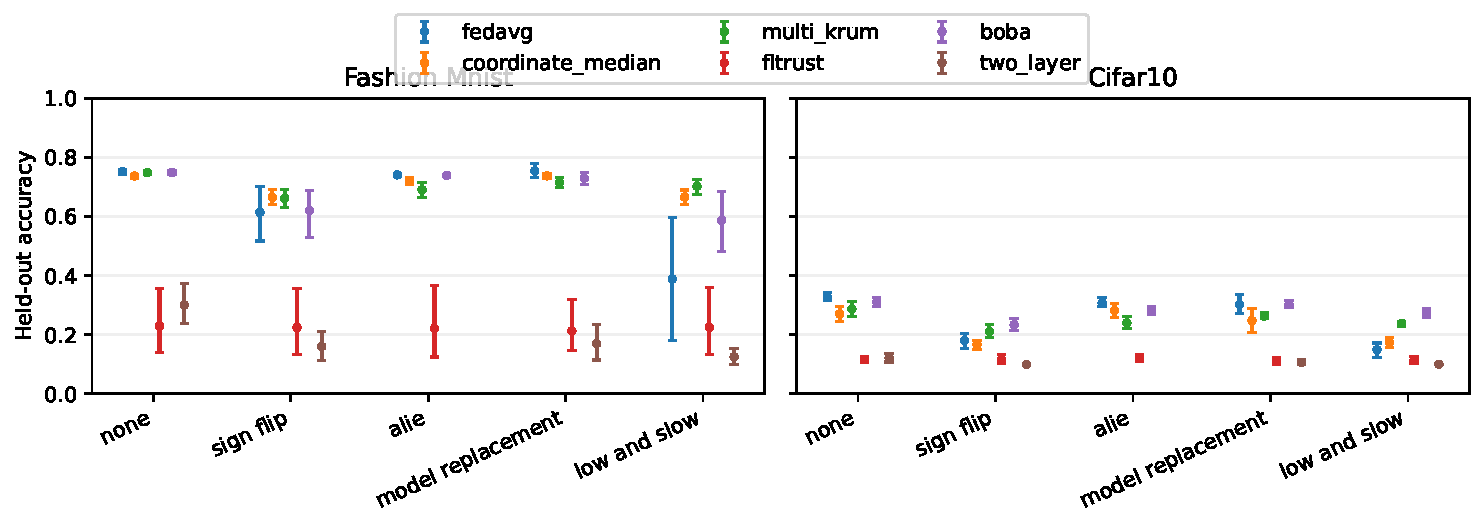
\includegraphics[width=0.95\textwidth]{figures/core_accuracy.pdf}
\caption{Matched core evaluation. Points show five-seed mean held-out accuracy; bars show bootstrap 95\% confidence intervals. Missing cells are incomplete or held, not zero-valued.}
\Description{Two dataset panels comparing complete five-seed groups across five attack conditions.}
\end{figure*}

\paragraph{Follow-up evidence status.}
No complete five-seed follow-up group is available. FedVal, FEMNIST, adaptive-attack and recovery-control results remain pending.

Implementation tests and local-EVM transactions establish execution of the
specified state machine. They do not establish robustness under real data,
large-scale Byzantine tolerance, privacy, or economic deterrence. The original
four/eight-client pilot and earlier synthetic diagnostics are excluded from
confirmatory tables. Completed development experiments are also excluded from
the confirmatory estimates.
The FedVal/FEMNIST extension is also pending. Its strengthened recovery
attestation rule is a protocol change, so original core outcomes are not
presented as validation of that rule. No result from a one-round runtime
preflight is included in robustness estimates.

The matched comparison table replaces cross-paper numerical rankings. Entries
are generated only after all five seeds for a cell have completed. Missing or
infeasible cells remain identifiable in the artifact status report. No zero-ASR
or zero-loss conclusion is drawn from a final-round acceptance counter.
